\section* {2.1  Методы простой итерации и Ньютона}

\subsection{Постановка задачи}
Реализовать методы простой итерации и Ньютона решения нелинейных уравнений в виде программ, задавая в качестве входных данных точность вычислений. С использованием разработанного программного обеспечения найти положительный корень нелинейного уравнения (начальное приближение определить графически). Проанализировать зависимость погрешности вычислений от количества итераций.

{\bfseries Вариант:} 12

$3^x-5x^2+1=0$
%\pagebreak

\subsection{Результаты работы}
\begin{figure}[h!]
\centering
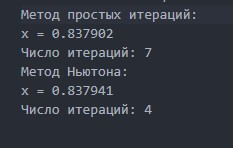
\includegraphics[width=12cm, height=6cm]{img1}
\caption{Вывод программы в консоли}
\end{figure}
\pagebreak

\subsection{Исходный код}
Файл с первым заданием второй лабораторной работы:
\lstinputlisting{include/task1.cpp}
\pagebreak

\section* {2.2  Методы простой итерации и Ньютона}

\subsection{Постановка задачи}
Реализовать методы простой итерации и Ньютона решения систем нелинейных уравнений в виде программного кода, задавая в качестве входных данных точность вычислений. С использованием разработанного программного обеспечения решить систему нелинейных уравнений (при наличии нескольких решений найти то из них, в котором значения неизвестных являются положительными); начальное приближение определить графически. Проанализировать зависимость погрешности вычислений от количества итераций. 

{\bfseries Вариант:} 12

\begin{cases}
& x_1-cos(x_2) = 3 \\
& x_2-sin(x_1) = 3 \\
\end{cases}
%\pagebreak

\subsection{Результаты работы}
\begin{figure}[h!]
\centering
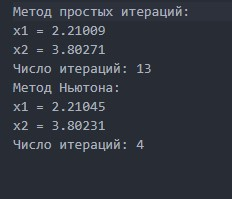
\includegraphics[width=15cm, height=6cm]{img2}
\caption{Вывод программы в консоли}
\end{figure}
\pagebreak


\subsection{Исходный код}
Файл со вторым заданием второй лабораторной работы:
\lstinputlisting{include/task2.cpp}